\chapter{Introduzione}
\label{chap:Introduction}
\glsresetall
In the last decades, the rapid growth of wireless technologies, dramatically increased the number of 
active mobile devices. Information collected or communicated by a wireless device is often meaningful 
only in conjunction with the knowledge of the device's location. For this reason, services and applications 
based on the knowledge of the user position, i.e.~\gls{lbs} have become of great interest, making
positioning an important requirement in modern wireless transmission systems \cite{Positioning_book1,Positioning_book2,Locating_the_nodes_cooperative_localization,Localization_via_ultra_wideband_radios_a_look}.
One of the leading applications of positioning techniques is transportation, including navigation, 
accident management, traffic routing and roadside assistance.
Another main application of civilian mobile positioning is safety. Indeed, strict  
positioning requirements have been demanded in order to satisfy legal mandates 
for location identification of emergency calls (e.g. E911 in US or E112 in Europe). 
Furthermore, \gls{lbs} are nowadays attracting in many fields, such as position-based advertising, 
personnel tracking, walk navigation assistance (in urban areas or inside buildings), 
position-dependent billing, 
and social networking applications. Finally, another class of services that has 
rapidly become popular is the pay-as-you-drive insurances \cite{Pay_as_you_drive_insurance}. 
Pay-as-you-drive vehicle insurance is a new type of car insurance that
ties the level of insurance premium to the risk level associated with the driving behavior of
the policyholder. If the driving is safe, i.e. the vehicle speed is appropriate for 
the type of street, the driver is rewarded with a premium reduction. 
The majority of \gls{lbs} requires accurate positioning for best operating.  
\glspl{gnss} greatly succeed to provide precise positioning of mobile devices in many 
environments. Nevertheless, GNSS receivers achieve poor performances in harsh 
environments, such as urban canyons or indoor areas, because of the sky view obstruction and 
because of the multipath propagation that is characteristic of such environments. 
Especially in these environments, terrestrial signals like the downlink signals of cellular networks 
or the beacons of WLAN access points may provide good coverage and may be used to determine the position 
of mobile terminals following an opportunistic approach.
Traditionally, cellular networks have provided support to improve the overall 
performance of \glspl{gnss}, as in the assisted-GNSS (A-GNSS), or to roughly estimate the user 
position by exploiting the knowledge of the cell identifier.
However, the localization precision that may be obtained with Cell-ID positioning depends on 
the cell coverage: for cellular networks in rural areas this may extend over several kilometers, 
while for WLANs it is in the order of hundreds of meters. A-GNSS offers significant performance 
advantages over autonomous GPS, but still suffer of sky obscuration 
that occurs in indoor environments. 
To achieve better performance in positioning with terrestrial signals, systems that exploits 
\gls{toa} ranging  time measurement-based may be employed. Indeed, these systems can can achieve 
great accuracy if the time estimations are correct.
The new emerging wireless standard \gls{3gpp} \gls{lte}, that is based on multicarrier signals is 
very attractive for this purpose. Indeed, LTE was explicitly designed with positioning capabilities by mean of a 
dedicated downlink signal that is referred to as \gls{prs}. Furthermore, other typical downlink signals of the
LTE standard like \gls{crs} can be exploited for \gls{toa} estimation, when the \glspl{prs} are not available.
The basic problem in time-based techniques is that the propagation delay of radio signal arriving from 
the direct path must be accurately estimated. However, in indoor environments and urban canyons, 
the direct path cannot always be accurately discriminated due to severe multipath propagation conditions.
Increasing the resolution of the channel estimation in order to distinguish paths that are received 
very close in time, may improve the performance of positioning systems based on time ranging. 
To address this issue, this thesis focused on the use of \glspl{sra}, which are a set of mathematical 
frameworks that may be used to estimate the time delays that characterize a multipath propagation 
channel. The name ``Super Resolution'' derives from the ability of these algorithms to resolve components 
that are very closely spaced in time or frequency.
In this thesis, a set of frameworks designed for estimating the \glspl{toa} of LTE reference 
signal was realized.
These frameworks make use of \glspl{sra} to improve the performances of \gls{toa}
estimation. The developed frameworks were then applied on real LTE data captured in a multipath scenario 
by the \gls{hsr} team, and on emulated LTE data which was kindly supplied by the \gls{dlr} team. 
To demonstrate their effectiveness, the performance of Super-Resolution techniques 
is compared with that of a conventional \gls{toa} estimation technique on emulated data. 
Moreover, the multipath scenario in which the real LTE data was captured, is simulated through a 
ray-tracing simulation software, and the resulting \glspl{toa} are compared with those calculated
using the proposed framework.
The first part of this thesis treats a theoretical background on positioning, LTE physical layer and \acrlongpl{sra}. The second part of the thesis analyzes in detail the developed frameworks, while in 
the rest of the thesis, results on the frameworks performances and a comparison with a conventional method 
are reported.

More specifically, the thesis is organized as follows.
\begin{itemize}
\item[-] Chapter \ref{chap:positioning} subsumes the most important ranging and positioning techniques, 
focusing on the signals' physical parameters that can be exploited for localization purposes.
\item[-] Chapter \ref{chap:lte_phisical_layer} describes the OFDM modulation system and the LTE 
standard physical layer. Moreover, the most important LTE synchronization and reference signals are 
described with the aim of providing a comprehensive background, that is needed for understanding the 
algorithms used in the remainder of the thesis. 
\item[-] Chapter \ref{chap:super_resolution_algorithms} analyzes the theory of \acrlongpl{sra}, 
that are widely used in the frameworks which are the subject of this thesis.
\item[-] Chapter \ref{chap:framework_toa_estimation} presents the developed frameworks 
for \gls{toa} estimation, classified as CRS based frameworks and PRS based frameworks. 
Moreover, a benchmark system not employing a \acrlongpl{sra} is described.
\item[-] Chapter \ref{chap:toa_estimation_real_data} reports the results obtained by applying  
the developed frameworks to real LTE data provided by the \gls{hsr} team. The performances 
obtained by each of the proposed frameworks are then compared in order to assessing 
the best tool to be used in realistic applications.
\item[-] Chapter \ref{chap:toa_estimation_emulated} reports the results obtained by applying the 
developed \gls{toa} estimation frameworks on emulated LTE data, that was acquired by the \gls{dlr} team. 
The results are reported in terms of root mean square error between the real and the estimated 
\glspl{toa}. Moreover, each framework is compared with the benchmark framework, 
to demonstrate the effectiveness of \glspl{sra} when employed on \gls{toa} estimation.
\item[-] Chapter \ref{chap:ray_tracing_simulation} describes the ray-tracing simulation tool 
Wireless InSite and reports the results of the simulation of an environment similar to the one
in which the real LTE data was captured. The \glspl{toa} calculated with this method are then 
compared to the \glspl{toa} obtained with the proposed frameworks.
\item[-] Finally, chapter \ref{chap:conclusions} summarizes the results obtained through this work and
proposes new ideas for future research studies.
\end{itemize}
This thesis work was accomplished in the Telecommunications Research Group at University of Trieste, 
under the supervision of Prof.~Fulvio Babich and Marco Driusso, who are gratefully acknowledged.

%\newpage\mbox{}\newpage


\includepdf[pages=-, offset = 0mm -0.9mm, pagecommand={}]{testi/SalutoBaldassa/salutoBaldassa.pdf}


\foreachpage{testi/lettera_fondazionale.pdf}{%
  \newpage   
  \begingroup 
    \centering
    \includegraphics[
      page=\value{imagepage},
      width=\textwidth,  
      height=\textheight,
    ]{testi/lettera_fondazionale.pdf}%
    \newpage
  \endgroup
}
